\chapter{4\quad Methodology}
\label{ch:methods}

\section{Social Network Analysis}
\label{sec:social_networks}

\subsection{Fundamentals}
\label{sec:social_networks_fundamentals}

In sociological terms, a social network is a social structure that maps out the relationships or interactions among various entities such as individuals, groups, organizations, or even entire societies. These entities, often referred to as nodes or vertices, are connected by one or multiple types of interdependencies, such as friendship, kinship, common interest, financial exchange, likes, dislikes, knowledge, prestige, or any other meaningful interactions or relationships.

Social networks are often visualized as graphs, where nodes represent the entities, and the edges or links represent the relationships or interactions between them. The patterns of these links often provide meaningful insights into the nature of relationships, social behaviours, group dynamics, organizational structures, and much more. For example, these structures may reveal who influences whom within a group or which entities act as gatekeepers or bridges in the flow of information or resources.

The size and complexity of social networks can vary greatly. They can be as small and simple as a family network or as vast and complex as the network of internet users across the globe. It's crucial to note that in a social network, the emphasis is on the relationships between entities, not just the entities themselves.

Graph theory, a fundamental area of mathematics, has found significant application in the study of social networks. In the context of social networks, graph theory provides a robust mathematical structure and a rich toolkit for understanding and analysing these networks.

A graph in mathematics is a structure that encapsulates the idea of pairwise relationships between objects. A graph comprises vertices (or nodes) and edges (or links). An edge connects a pair of vertices, indicating a relationship between them. This simple but powerful concept fits perfectly with the idea of a social network where entities (vertices) and their relationships (edges) form the fabric of the network. To make a formal definition, a basic social network can be defined as a tuple $G = (V,E)$, where $V$ is the set of vertices, and $E \subseteq V \times V$ is the set of edges.

\bigskip
\noindent Social network analysis (SNA) often leverages graph theory in multiple ways:

\begin{itemize}
	\item Visualisation: Graph theory aids in visually representing social networks, enabling a clear understanding of the complex web of relationships.
	\item Measurement and Analysis: Graph theory provides various measures and metrics such as centrality, clustering coefficient, diameter, etc., which can quantify important aspects of social networks like prominence of entities, propensity of clustering, reachability, etc.
	\item Modelling and Prediction: Graph models can mimic the behaviour of real-world social networks, helping in predicting future trends, understanding the spread of information or epidemics, or identifying influential entities in the network.
	\item Community Detection: Algorithms derived from graph theory help to discover communities or clusters within networks, revealing groups of entities with densely packed relationships.
\end{itemize}

\noindent In summary, a social network is a social structure that portrays interactions or relationships among entities. These networks can be effectively represented, measured, analysed, and modelled using the concepts and tools provided by graph theory, which provides a powerful mathematical lens to understand the complex dynamics of social networks. 

\subsection{Application to COVID-19 case contact data}
\label{sec:social_networks_application}

As mentioned earlier, social networks can be used to model the social dynamics of pandemic situations. Recall the definition of a social network as a tuple $G = (V,E)$. All datasets analysed in this work adhere to the basic form (time, source, target), and additional covariates depending on the dataset in question. The time component can be discarded for now, as it becomes relevant only when working with relational (hyper)event models later on. In the context of case contact networks, $V$ therefore is the set of cases/contacts, and $E$ is the set of contact nominations between cases. One might make a case for using bipartite (also known as two-mode networks), where vertices are divided into two classes, and edges only exist between vertices of different class \cite{borgatti1997network,latapy2008basic}. Although it may seem sensible to do this here, where, in principle, there are indeed two classes (nominators and nominees), in practice, this only holds true for the data from Bucharest, where a large fraction of nominated contacts were never registered as positive cases. However, it is not clear if this is only due to missing information, i.e. they might have contracted the virus and health authorities were just not aware of it, or due to them indeed not having been infected. Therefore, and to ensure comparability of results, two-mode networks were not used to model the case contact networks here. 

Also, there is the question of directionality. Networks can be either directed or undirected, meaning that edges between nodes $u$ and $v$ are either one- or bidirectional. Directed networks usually carry a different semantic meaning compared to undirected ones, and also differ in the computation of network effects. For example, in a directed network, nodes have an in-degree and an out-degree, i.e. the number of incoming and outgoing edges, respectively; therefore, there also need to be two measures for degree centrality, one accounting for in-degree, and one for out-degree. Although it might seem sensible to use directed networks here, since contact nominations are of a (source, target) form, the actual semantic meaning of the connection is often not clear (i.e. whether the source node is naming possible contacts who might have infected him, or if the source node is naming contacts whom he himself might have infected) \cite{kojaku2021effectiveness}, except for the Bucharest dataset, where it is explicitly stated that authorities employed backward contact tracing, i.e. patients name individuals who might be the source of their infection \cite{hancean2021role}.

\subsection{Network analysis}
\label{sec:social_networks_analysis}

As mentioned in section \ref{sec:social_networks_fundamentals}, graph theory offers a wide array of methods to extract useful information from social networks. In the context of pandemics, key interests include the identification of influential individuals (e.g. "super-spreaders") and the overall dynamic of infections, i.e. in which patterns a virus tends to spread; insights into these factors help understanding, and therefore combatting the respective pandemic, e.g. by putting a particular focus on individuals who are similar to those found to be especially prone to spread the virus to others \add{cite}.

For all networks derived from the different datasets, the following network statistics were computed:

\begin{itemize}
	\item Degree centrality: For any node $v \in V$, the degree centrality is defined as $C_D(v) = \frac{\text{deg}(v)}{\lvert V \rvert - 1}$, i.e. the degree centrality of a node is equal to the number of edges connected to that node, normalised by the maximum possible degree in the graph, i.e. the total number of nodes minus one. This measure can be used to identify individuals who hold an important position in the network (in this context, those who nominate many contacts), and also as an indicator for overall network density.
	\item Betweenness centrality: For any node $v \in V$, the betweenness centrality is defined as $C_B(v) = \sum_{s\neq v\neq t\in V}\frac{\sigma_{st}(v)}{\sigma_{st}}$, where $\sigma_{st}$ is the total number of shortest paths from $s$ to $t$, and $\sigma_{st}(v)$ is the number of shortest paths from $s$ to $t$ that go through $v$. This measure can be used to identify individuals who facilitate information flow (in this context, those who might have spread the virus from one individual to another).
	\item Pagerank centrality: This is an iterative algorithm originally proposed to rank websites according to importance, where importance is defined by the number of hyperlinks that point to that website. For any node $v \in V$, the pagerank centrality is defined as $C_P(v) = \sum_{u \in B_v}\frac{C_P(u)}{\text{deg}(u)}$, where $B_v$ is the set of all nodes connected to $v$. Pagerank is computed iteratively; at time 0, it is
	\begin{equation*}
		PR(v_i;0) = \frac{1}{N} \forall v_i \in V
	\end{equation*}
	where $N = \lvert V \rvert$. At time $t$, it is
	\begin{equation*}
		PR(v_i;t+1) = \frac{1 - d}{N} + d \sum_{v_j \in B_{v_i}} \frac{PR(v_j;t)}{deg(v_j)} \forall v_i \in V
	\end{equation*}
	where $d = 0.85$ is the damping parameter. This measure is another way to identify important individuals in the network.
	\item Component size: The task of community detection is the division of a network into a set of sub-networks according to specific criteria; in general, a community is a set of nodes with a strong cohesion, i.e. a high degree of inter-connectedness, while connections to other groups are sparse or even non-existent. Here, the latter is the case, i.e. a connected component is a set of nodes $C = \{v_1,...,v_n\} \in V$, where for each pair of nodes $v_i,v_j \in C$, there exists an edge $(v_i,v_j) \in E$, and for each pair $v_i,n_j;\: v_i \in C, n_j \in V \setminus C$, there is no edge, i.e. $(v_i,n_j) \notin E$. This division can be achieved e.g. by \emph{Markov clustering algorithm} \cite{community_detection,markov_clustering}. In the context of pandemics, community detection can be used to identify infection clusters. Therefore, connected components are computed for all networks, and component size is determined for all nodes.
	\item Average shortest path length: In general, the shortest path between any two nodes $v_x,v_y \in V$ is a sequence of vertices $S = (v_x,...,v_y)$ such that 
	\begin{enumerate}
		\item for all $v_i,v_j \in S, i < j$, there is an edge $(v_i,v_j) \in E$
		\item out of all possible paths between $v_x$ and $v_y$, $S$ has the smallest cost
	\end{enumerate}
	where cost is the sum of weights associated with the edges. Since the graphs here are unweighted, i.e. all edges have a weight value of 1, the shortest path amounts to that sequence $S$ that contains the lowest amount of nodes out of all possible sequences. Shortest paths can be computed for example by the Dijkstra or A* algorithm \add{cite dijsktra, a* and shortest path definition}. In the context of case contact networks, shortest paths yield interesting insights into transmission chains, and the average shortest path length of a network might be used as a measure for how effective containment methods (e.g. lockdowns, social distancing etc.) have been.
\end{itemize}  
\bigskip

\noindent Based on these statistics, the data was analysed both in qualitative and quantitative manner. Specifically, examples are given for how epidemiological insights can be gained from contact tracing data (qualitative), and the statistics computed for the different datasets are statistically compared to investigate whether there are significant differences between the different regions (quantitative). Furthermore, ordinary least-squares regression models are used to determine the influence of node-specific network statistics and actor covariates on contact nomination likelihood. Results are presented in section \ref{ch:results_discussion}.

\section{Relational Event Models}
\label{sec:rem}

\subsection{Fundamentals}
\label{sec:rem_fundamentals}

Relational event models (REMs) are a class of statistical models used for analysing ordered sequences of social interactions among actors. They offer a means to explain the timing and sequencing of events in a social network context, often focusing on patterns of communication, relationships, and interactions between network actors over time. 

In the realm of social networks, an event signifies an action that happens at a specific point in time from one actor to another. For instance, in a network of email communications among a group of people, an email sent by person A to person B would be considered an event. REMs are concerned with the study of these actions or events, their timing, and the dependencies between them.

The main idea behind REMs is to treat social interactions as events that happen in continuous time, rather than at discrete, predetermined intervals. Each event in the sequence is an interaction between pairs of actors, and the time between consecutive events is explicitly modelled and analysed. 

\noindent REMs take into consideration two key factors:

\begin{enumerate}
	\item Order of events: The order in which events occur can have significant implications. For example, an email conversation would make little sense if the emails are not read in the sequence they were sent and received.
	\item Timing of events: The time between consecutive events can reveal crucial information. For example, the length of time between receiving an email and replying to it could indicate the importance or urgency of the conversation.
\end{enumerate}

REMs use the order and timing information to make inferences about the underlying social process that generated the observed sequence of events. They allow for the analysis of dynamic network data in ways that conventional social network analysis tools, which often assume static networks, can not. 

Applications of REMs include studying patterns of communication in social media, organisational behaviour, group dynamics, online collaboration, animal social behaviour, and many other fields where understanding the sequence and timing of interactions can provide valuable insights.

In essence, relational event models specify the probability of a possible event sequence $E$ happening up to a point in time $t_n$, given a sequence of past events $E_{<t_n}$; formally, it is
\begin{equation*}
	P(E) = \prod_{i=1}^{n}P(e_i|E_{<t_i})
\end{equation*}
where $E = (e_1,...,e_n)$ is a sequence of events, and $E_{<t_i} = \{e_j \in E;\: t_j < t_i\}$ is the sequence of past events before $t_i$.

The partial likelihood for a specific event $e_i = (u_i,v_i,t_i)$, which is an interaction from $u_i$ to $v_i$ ($u_i,v_i \in A$, i.e. $A = U \cup V$ is the set of all actors; $U$ and $V$ are the not necessarily disjoint sets of sources and targets) is expressed in terms of hazard functions. It is
\begin{equation*}
	P(e_i|E_{<t_i};\theta) = \frac{\lambda(u_i,v_i,t_i;\theta)}{\sum_{uv\in R_{t_i}}\lambda(u,v,t_i;\theta)}
\end{equation*}
where $\lambda(u,v,t_i;\theta)$ is the hazard rate of the dyad $(u,v)$, i.e. the expected number of events on $(u,v)$ per time unit, and $R_{t_i}$ is the set of all events that could potentially happen at time $t_i$, aka the risk set. The rate function $\lambda$ depends on source ($u$), target ($v$), event type, past event history ($E_{<t_i}$), and exogenous variables. It is given by
\begin{align*}
	\lambda(u,v,t_i;\theta) = \lambda_0(t_i) \cdot \lambda_1(u,v,t_i;\theta)
\end{align*}
i.e. it is decomposed into an arbitrary baseline rate $\lambda_0$ and a parametrised relative rate $\lambda_1$:
\begin{align*}
	\lambda_1(u,v,t_i;\theta) &= \exp(\theta^T s(u,v;E_{<t_i}))\\
	&= \exp(\sum_h \theta_h \cdot s_h(u,v;E_{<t_i}))&&
\end{align*}
This is expressed by a vector of statistics $s$, which is parametrised by a vector of unknown parameters ($\theta$, estimated from the data), which determine the influence of each individual factor on the overall incidence rate. To summarise, the probability for a particular event $e_i$ occurring is the hazard rate of $e_i$ divided by the sum of the hazard rates of all events which could potentially occur at time $t_i$ \cite{butts20084}.

The statistics expressed by $s$ may be broadly categorised into endogenous and exogenous factors; endogenous factors are derived from past events involving $u$ and $v$, and possibly common third actors, while exogenous factors are given by covariates specific to the actors, e.g. personal characteristics like age or sex. 

Given a set of sufficient statistics $s$, the model parameters $\theta$ can be determined through maximum likelihood estimation (MLE), such that \[\hat{\theta} = \argmax_{\theta} P(E|\theta)\]

A potential issue in this MLE is the computation of the risk set $R$; this is because the number of potential events occurring at time $t_i$ rises quadratically with the number of actors (with $N$ actors, for each time step $t_i$, there are $N \cdot (N - 1)$ possible events) \cite{butts20084}. This can be alleviated by replacing the full risk set $R_{t_i}$ by a sampled risk set $\tilde{R_{t_i}}$, which contains an arbitrary number of potential events per observed event (e.g. 100 potential, but unobserved events per every one event seen in the data), which are sampled uniformly at random \cite{eventnet_rem}.

\subsection{Application to COVID-19 case contact data}
\label{sec:rem_application}

Recall that all case contact datasets conform to the basic format (timestamp, source, target). Therefore, they are, in essence, sequences of events, where the social interaction between the actors is a contact nomination. Conventional social network analysis, as described in section \ref{sec:social_networks}, neglects the time component of the data entirely. Therefore, it seems prudent to also analyse the data using relational event modelling. It is worthy to note that, in contrast to static network modelling, REM necessitates an assumption of directionality, i.e. events have a source and a target; in this case, the source would be the nominator, and the target the nominee. However, the fact remains that it is difficult to determine the actual semantic of a particular interaction, i.e. whether the source infected the target, or vice versa.

As mentioned before, there are essentially two steps, which are 1) the computation of statistics $s$, and 2) the estimation of model parameters $\theta$. Therefore, it is necessary to specify a set of statistics which may potentially influence the incidence rate of events. Based on previous work (\cite{butts20084,brandes2009networks,stadtfeld2017interactions}), the following effects were analysed:

\begin{figure}
	\centering
	\begin{subfigure}[t]{0.2\linewidth}
		\vskip 0pt
		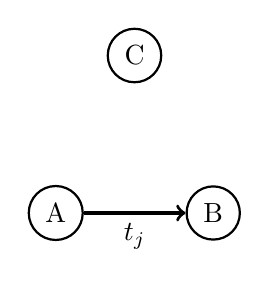
\begin{tikzpicture}
			\begin{scope}[every node/.style={circle,thick,draw}]
				\node (A) at (0,0) {A};
				\node (B) at (2,0) {B};
				\node (C) at (1,2) {C};
			\end{scope}
			
			\begin{scope}[every edge/.style={draw=black,very thick}]
				\path [->] (A) edge node [below] {$t_j$} (B);
				%\path (B) edge node {} (C);
				%\path (C) edge node {} (A);
			\end{scope}
		\end{tikzpicture}
		\caption{Event $(A,B,t_j)$}
	\end{subfigure}
	\hfill
	\begin{subfigure}[t]{0.2\linewidth}
		\vskip 0pt
		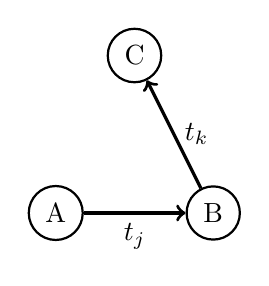
\begin{tikzpicture}
			\begin{scope}[every node/.style={circle,thick,draw}]
				\node (A) at (0,0) {A};
				\node (B) at (2,0) {B};
				\node (C) at (1,2) {C};
			\end{scope}
			
			\begin{scope}[every edge/.style={draw=black,very thick}]
				\path [->] (A) edge node [below] {$t_j$} (B);
				\path [->] (B) edge node [right] {$t_k$} (C);
				%\path (C) edge node {} (A);
			\end{scope}
		\end{tikzpicture}
		\caption{Event $(B,C,t_k)$}
	\end{subfigure}
	\hfill
	\begin{subfigure}[t]{0.2\linewidth}
		\vskip 0pt
		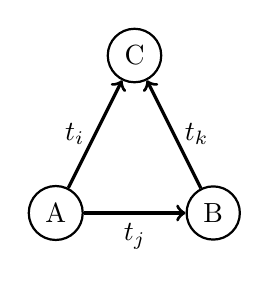
\begin{tikzpicture}
			\begin{scope}[every node/.style={circle,thick,draw}]
				\node (A) at (0,0) {A};
				\node (B) at (2,0) {B};
				\node (C) at (1,2) {C};
			\end{scope}
			
			\begin{scope}[every edge/.style={draw=black,very thick}]
				\path [->] (A) edge node [below] {$t_j$} (B);
				\path [->] (B) edge node [right] {$t_k$} (C);
				\path [->] (A) edge node [left] {$t_i$} (C);
			\end{scope}
		\end{tikzpicture}
		\caption{Transitive closure through event $(A,C,t_i)$}
	\end{subfigure}
	\hfill
	\begin{subfigure}[t]{0.2\linewidth}
		\vskip 0pt
		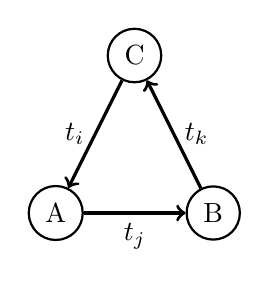
\begin{tikzpicture}
			\begin{scope}[every node/.style={circle,thick,draw}]
				\node (A) at (0,0) {A};
				\node (B) at (2,0) {B};
				\node (C) at (1,2) {C};
			\end{scope}
			
			\begin{scope}[every edge/.style={draw=black,very thick}]
				\path [->] (A) edge node [below] {$t_j$} (B);
				\path [->] (B) edge node [right] {$t_k$} (C);
				\path [->] (C) edge node [left] {$t_i$} (A);
			\end{scope}
		\end{tikzpicture}
		\caption{Cyclical closure through event $(C,A,t_i)$}
	\end{subfigure}
	\caption{Illustration of transitive and cyclical closure in relational event models. Time ordering is $t_j < t_k < t_i$.}
	\label{fig:rem_closure}
\end{figure}

\begin{itemize}
	\item Effects depending on past events:
	\begin{itemize}
		\item Nomination activity, i.e. the influence of the number of past events at times $<t_i$ involving actor $u$ as a source on the likelihood a possible event $(u,v,t_i)$ $\rightarrow$ is the nomination activity of $u$ associated with the likelihood of a future event on the dyad $(u,v)$?
		\begin{align*}
			&nomination.activity(e(u,v,t_i)) = \sum_{v' \in V} e(u,v',<t_i)&&\\
			&nomination.activity(e(u,v,t_i)) = \lvert E' \rvert; E' = \{e(u,v',t_j) \forall v' \in V \land t_j < t_i\}
		\end{align*}
		\item Exact repetition, i.e. the influence of the number of past events $(u,v,<t_i)$ on the likelihood of a possible event $(u,v,t_i)$ $\rightarrow$ is the likelihood of a future event on the dyad $(u,v)$ associated with the number of past observed events on the same dyad?
		\begin{align*}
			exact.repetition(e(u,v,t_i)) = \sum e(u,v,<t_i)
		\end{align*}
		\item Reciprocation, i.e. the influence of the number of past events $(x,u,<t_i)$ on the likelihood of a possible event $(u,v,t_i)$ $\rightarrow$ is the number of times $u$ has been named as a contact in the past associated with the likelihood of a future event on the dyad $(u,v)$, i.e. $u$ now acting as a nominator himself?
		\begin{align*}
			reciprocation(e(u,v,t_i)) = \sum_{u' \in U} e(u',u,<t_i)
		\end{align*}
		\item Exact reciprocation, i.e. the influence of the number of past events $(v,u,<t_i)$ on the likelihood of a possible event $(u,v,t_i)$ $\rightarrow$ is the number of past events on the dyad $(v,u)$ associated with the likelihood of a future event involving the same actors, but with roles reversed?
		\begin{align*}
			exact.reciprocation(e(u,v,t_i)) = \sum e(v,u,<t_i)
		\end{align*}
		\item Transitive tie, i.e. the influence of past events $(u,x,t_j)$ and $(x,v,t_k)$, $j < k < i$ on the likelihood of a possible event $(u,v,t_i)$ $\rightarrow$ is there a tendency for transitive closure?
		\begin{align*}
			transitive.tie(e(u,v,t_i)) = \sum_{x=1}^{\lvert \mathcal{R} \rvert} \min [d(u,x,A_{t_i}), d(x,v,A_{t_i})]
		\end{align*}
		($\mathcal{R}$ is the set of potential targets; $d(x,y,A_{t_i})$ is the accumulated volume of interactions from $x$ to $y$ by the time $t_i$)
		\item Cyclical tie, i.e. the influence of past events $(u,x,t_j)$ and $(x,v,t_k)$, $j < k < i$ on the likelihood of a possible event $(v,u,t_i)$ $\rightarrow$ is there a tendency for cyclical closure? (for an illustration, refer to figure \ref{fig:rem_closure})
		\begin{align*}
			cyclical.tie(e(u,v,t_i)) = \sum_{x=1}^{\lvert \mathcal{R} \rvert} \min [d(v,x,A_{t_i}), d(x,u,A_{t_i})]
		\end{align*}
		\item Shared source, i.e. the influence of the number of past events $(x,u,t_j)$ and $(x,v,t_k)$, $j \leq k < i$ on the likelihood of a possible event $(u,v,t_i)$ or $(v,u,t_i)$ $\rightarrow$ is there a tendency for actors who have been nominated as contacts by the same individual to name each other as contacts at a later time? (for an illustration, refer to figure \ref{fig:rem_triangle_children})
		\begin{align*}
			shared.source(e(u,v,t_i)) = \sum_{x=1}^{\lvert \mathcal{R} \rvert} \min [d(x,u,A_{t_i}), d(x,v,A_{t_i})]
		\end{align*}
		\item Shared target, i.e. the influence of the number of past events $(u,x,t_j)$ and $(v,x,t_k)$, $j \leq k < i$ on the likelihood of a possible event $(u,v,t_i)$ or $(v,u,t_i)$ $\rightarrow$ is there a tendency for actors who have nominated the same individual as a contact to name each other as contacts at a later time? (for an illustration, refer to figure \ref{fig:rem_triangle_parents})
		\begin{align*}
			shared.sender(e(u,v,t_i)) = \sum_{x=1}^{\lvert \mathcal{R} \rvert} \min [d(u,x,A_{t_i}), d(v,x,A_{t_i})]
		\end{align*}
	\end{itemize}
	\item Effects depending on actor attributes:
	\begin{itemize}
		\item Nominator age
		\item Nominee age
		\item Age difference between nominator and nominee (age homophily)
		\item Nominator sex
		\item Nominee sex
		\item Sex difference between nominator and nominee (sex homophily)
		\item Other covariates specific to the individual datasets, which are listed in section \ref{ch:previous_work_data}. In general, there are three statistics for each covariate: the value of the nominator, the value of the nominee, and the difference between the values.
	\end{itemize}
\end{itemize}

\begin{figure}
	\centering
	\begin{subfigure}[t]{0.3\linewidth}
		\vskip 0pt
		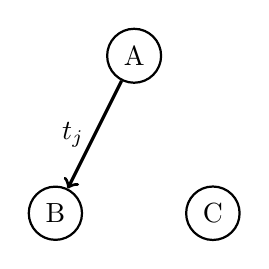
\begin{tikzpicture}
			\begin{scope}[every node/.style={circle,thick,draw}]
				\node (A) at (1,2) {A};
				\node (B) at (0,0) {B};
				\node (C) at (2,0) {C};
			\end{scope}
			
			\begin{scope}[every edge/.style={draw=black,very thick}]
				\path [->] (A) edge node [left] {$t_j$} (B);
				%\path (B) edge node {} (C);
				%\path (C) edge node {} (A);
			\end{scope}
		\end{tikzpicture}
		\caption{Event $(A,B,t_j)$}
	\end{subfigure}
	\hfill
	\begin{subfigure}[t]{0.3\linewidth}
		\vskip 0pt
		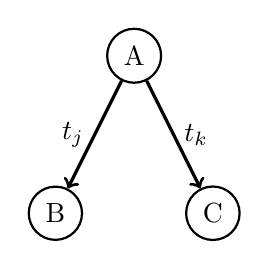
\begin{tikzpicture}
			\begin{scope}[every node/.style={circle,thick,draw}]
				\node (A) at (1,2) {A};
				\node (B) at (0,0) {B};
				\node (C) at (2,0) {C};
			\end{scope}
			
			\begin{scope}[every edge/.style={draw=black,very thick}]
				\path [->] (A) edge node [left] {$t_j$} (B);
				\path [->] (A) edge node [right] {$t_k$} (C);
				%\path (C) edge node {} (A);
			\end{scope}
		\end{tikzpicture}
		\caption{Event $(B,C,t_k)$}
	\end{subfigure}
	\hfill
	\begin{subfigure}[t]{0.3\linewidth}
		\vskip 0pt
		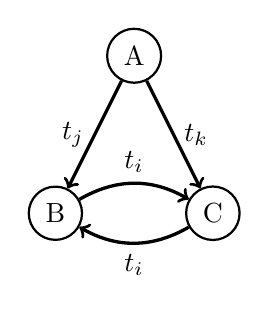
\begin{tikzpicture}
			\begin{scope}[every node/.style={circle,thick,draw}]
				\node (A) at (1,2) {A};
				\node (B) at (0,0) {B};
				\node (C) at (2,0) {C};
			\end{scope}
			
			\begin{scope}[every edge/.style={draw=black,very thick}]
				\path [->] (A) edge node [left] {$t_j$} (B);
				\path [->] (A) edge node [right] {$t_k$} (C);
				\path [->] (B) edge [bend left] node [above] {$t_i$} (C);
				\path [->] (C) edge [bend left] node [below] {$t_i$} (B);
			\end{scope}
		\end{tikzpicture}
		\caption{Shared source through event $(A,C,t_i)$}
	\end{subfigure}
	\hfill
	\caption{Illustration of shared source in relational event models. Time ordering is $t_j \leq t_k < t_i$.}
	\label{fig:rem_triangle_children}
\end{figure} 

\begin{figure}
	\centering
	\begin{subfigure}[t]{0.3\linewidth}
		\vskip 0pt
		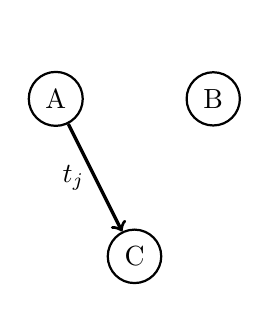
\begin{tikzpicture}
			\begin{scope}[every node/.style={circle,thick,draw}]
				\node (A) at (0,2) {A};
				\node (B) at (2,2) {B};
				\node (C) at (1,0) {C};
			\end{scope}
		
			\begin{scope}[every edge/.style={very thick}]
				\path [->] (A) edge [bend left] node [above,style={text opacity=0}] {$t_i$} (B);
				\path [->] (B) edge [bend left] node [below] {} (A);
			\end{scope}
			
			\begin{scope}[every edge/.style={draw=black,very thick}]
				\path [->] (A) edge node [left] {$t_j$} (C);
				%\path (B) edge node {} (C);
				%\path (C) edge node {} (A);
			\end{scope}
		\end{tikzpicture}
		\caption{Event $(A,B,t_j)$}
	\end{subfigure}
	\hfill
	\begin{subfigure}[t]{0.3\linewidth}
		\vskip 0pt
		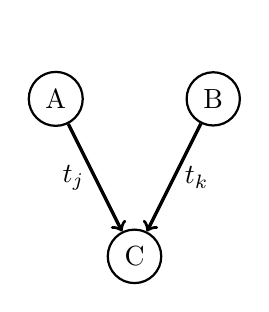
\begin{tikzpicture}
			\begin{scope}[every node/.style={circle,thick,draw}]
				\node (A) at (0,2) {A};
				\node (B) at (2,2) {B};
				\node (C) at (1,0) {C};
			\end{scope}
		
			\begin{scope}[every edge/.style={very thick}]
				\path [->] (A) edge [bend left] node [above,style={text opacity=0}] {$t_i$} (B);
				\path [->] (B) edge [bend left] node [below] {} (A);
			\end{scope}
			
			\begin{scope}[every edge/.style={draw=black,very thick}]
				\path [->] (A) edge node [left] {$t_j$} (C);
				\path [->] (B) edge node [right] {$t_k$} (C);
				%\path (C) edge node {} (A);
			\end{scope}
		\end{tikzpicture}
		\caption{Event $(B,C,t_k)$}
	\end{subfigure}
	\hfill
	\begin{subfigure}[t]{0.3\linewidth}
		\vskip 0pt
		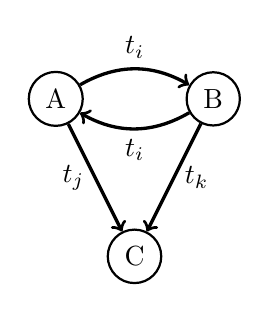
\begin{tikzpicture}
			\begin{scope}[every node/.style={circle,thick,draw}]
				\node (A) at (0,2) {A};
				\node (B) at (2,2) {B};
				\node (C) at (1,0) {C};
			\end{scope}
			
			\begin{scope}[every edge/.style={draw=black,very thick}]
				\path [->] (A) edge node [left] {$t_j$} (C);
				\path [->] (B) edge node [right] {$t_k$} (C);
				\path [->] (A) edge [bend left] node [above] {$t_i$} (B);
				\path [->] (B) edge [bend left] node [below] {$t_i$} (A);
			\end{scope}
		\end{tikzpicture}
		\caption{Shared target through event $(A,C,t_i)$}
	\end{subfigure}
	\hfill
	\caption{Illustration of shared target in relational event models. Time ordering is $t_j \leq t_k < t_i$.}
	\label{fig:rem_triangle_parents}
\end{figure}

These statistics were calculated using the \emph{eventnet} software \cite{eventnet_rem,eventnet_rhem} (step 1). Using the \emph{R} package \emph{survival} \cite{survival-package}, a Cox proportional hazards model was fitted on the result tables in order to estimate the model parameters $\theta$, and therefore draw conclusions regarding significance and effect of the individual statistics (step 2). Results are presented and discussed in chapter \ref{ch:results_discussion}.

\section{Relational Hyperevent Models}
\label{sec:rhem}

\subsection{Fundamentals}
\label{sec:rhem_fundamentals}

A limiting factor for relational event modelling is the restriction to dyadic interactions; while many events involve not only two but multiple actors (e.g. an email sent to a mailing list containing multiple recipients), these events are treated independently of one another in REM. This negligence of possible dependencies between targets may lead to erroneous parameter estimations. For example, take a possible event $(A,B,t_i)$, where Alice sends an email to Bob at time $t_i$. There is also a history of past interactions $(A,B,t_j)$ and $(A,C,t_j); t_i < t_j$, where Alice sent an email addressing both Bob and Charlie. A relational event model containing a \emph{repetition} statistic would find a positive effect for this interaction, while in reality, Alice might always send emails addressed to both Bob and Charlie, but never to Bob alone, so an event $(A,B,t_i)$ would actually be a novelty instead of a repetition. 

Perry and Wolfe \cite{perry2013point} propose an adjusted formula for the intensity rate
\begin{align*}
	&\lambda(u,J,t_i;\theta) = \lambda_0(t_i) \cdot \lambda_1(u,J,t_i;\theta)&&\\
	&\lambda_1(u,J,t_i;\theta) = \exp(\theta^T \sum_{j\in J} s(u,j;E_{<t_i})) \prod_{j\in J} \mathbf{1}\{j \in \mathcal{J}_{t_i} (u)\} \add{what is meant by last part?}&&
\end{align*}
where $u$ is the source of the interaction, $J$ is the set of targets of the interaction, and $\mathcal{J}_{t_i} (u)$ is the set of all possible targets of $u$ at time $t_i$. This model therefore assumes that covariate vectors $s$ of recipients $j \in J$ influence the intensity rate for an event $(u,J,t_i)$ independently of one another, since intensity of a multicast interaction is expressed through a decomposition into dyadic interactions \cite{perry2013point,lerner2021relational}.

Other approaches include the creation of artificial nodes that contain the receiver set (refer to figure \ref{fig:polyadic_interactions}) and the employment of hyperedge or latent variable models; issues with these are a possibly intractable amount of receiver set nodes in the first case, and limitation to dyadic functions in the latter two cases \cite{lerner2021relational}. 
\bigskip

\noindent Lerner et al \cite{lerner2019rem} propose a generalisation of relational event models based on hypergraphs. Hypergraphs are an extension of traditional graphs, where edges can not only connect two, but any number of nodes; formally, a hypergraph is defined by a tuple $H = (V, E)$, where $V$ is the set of vertices, and $E \subseteq 2^V$ is a set of non-empty subsets of $V$, i.e. the hyperedges. A directed hypergraph is defined by a triplet $H = (U,V,E)$, where $U$ (= sources) and $V$ (= targets) are sets of vertices, and $E \subseteq 2^U \times 2^V$ is a set of tuples $h = (u,v)$, where $u \in U$ is a non-empty set of source vertices, and $v \in V$ is a non-empty set of target vertices \cite{wang2018development,lerner2019rem}. Henceforth, only the directed case shall be considered.

Based on the concepts of REM, a directed hyperevent is given by $e_i = (h_i, t_i, x_i)$, where $h_i$ is a directed hyperedge, $t_i$ is a point in time when the event takes place, and $x_i$ is the type of the event (e.g. sending an email); the latter component will be neglected as it is not relevant to this work. Similarly, the hazard rate is given by
\begin{align*}
	&\lambda(h,t_i,\theta) = \theta_0(t_i) \cdot \lambda_1(h,t_i;\theta)&&\\
	&\lambda_1(h,t_i;\theta) = \exp(\theta^T s(h;E_{<t_i}))
\end{align*}
and the partial likelihood of an event sequence is given by 
\begin{align*}
	L(\theta) = \prod_{e \in E_{<t_i}} \frac{\lambda_1(h_e,t_e;\theta)}{\sum_{h\in R_{t_e}} \lambda_1(h,t_e;\theta)}
\end{align*}
Compared to the approach by Perry and Wolfe, the only difference is the substitution of the decomposition of statistic vectors $\sum_{j} s(u,j;E_{<t_i})$ for a hyperedge vector $s(h;E_{<t_i})$ \cite{lerner2019rem,lerner2021relational}. Apart from that, the computation of the risk set $R$ poses an even greater problem than it does for relational event models. This is because all possible hyperedges need to be considered, the number of which rises exponentially with the number of nodes. Like before, case-control sampling is used to reduce the risk set to a tractable size \cite{lerner2019rem,lerner2021relational}.
\bigskip

\noindent The main novelty, therefore, is the definition of the statistics $s$.

\subsection{Application to COVID-19 case contact data}
\label{sec:rhem_application}

Obviously, most contact nomination events are not dyadic, but polyadic, i.e. multiple actors are involved; think, for example, of a birthday party, after which one of the attendees tests positive and names all other guests as contacts. Therefore, conventional relational event models may fail to identify dynamics due to their dyadic nature. As stated in the previous section, a directed hyperevent generally consists of a non-empty set of source actors $u$ and target actors $v$; since in all datasets used in this work there is always a single COVID-19 patient nominating one or more contacts, it is $\lvert u \rvert$ for all hyperevents, i.e. there is only one source actor. For this reason, directed RHEM were chosen instead of undirected.

The statistics included in the models are in part similar to the ones used in REM, but differ in their definition. Once again, they can be divided into endogenous and exogenous effects, i.e. statistics depending on prior events, and statistics depending on actor covariates. Based on previous work (\cite{lerner2019rem,lerner2021relational,hancean2021role,hancean2022occupations}), the following were analysed:

\begin{itemize}
	\item Effects depending on past events:
	\begin{itemize}
		\item Nominee set size, i.e. the influence of the size of the target set of a hyperedge $h$ involved in past events $e(h,<t_i)$ at times $<t_i$ on the likelihood of a possible event $e(h,t_i)$ $\rightarrow$ is the number of named contacts associated with the likelihood of future events?
		\begin{align*}
			nominee.size(e(h,t_i)) = \lvert v \rvert; \: h = (u,v)
		\end{align*}
		\item Exact repetition, i.e. the influence of the number of past events $e(h,<t_i)$ on the likelihood of a possible event $e(h,t_i$) $\rightarrow$ is the number of past events on a hyperedge $h$ associated with the likelihood of a future event on the exact same hyperedge?
		\begin{align*}
			exact.repetition(e(h,t_i)) = \sum e(h,<t_i)
		\end{align*}
		\item Unordered repetition, i.e. the influence of the number of past events $e(h',<t_i)$ on the likelihood of a possible event $e(h,t_i)$, where $h' = (u',v'); \: h = (u,v); \: u',v' \in u \cup v$ $\rightarrow$ is the likelihood of a future event $e(h,t_i)$ associated with the number of past events on hyperedges which contain the same actors, but not necessarily in the same roles?
		\begin{align*}
			unordered.repetition(e(h,t_i)) = \sum e(h',<t_i); \: h.source \cup h.targets = h'.source \cup h'.targets
		\end{align*}
		\begin{figure}
			\begin{mdframed}
				\centering
				\begin{subfigure}[t]{0.45\linewidth}
					\vskip 0pt
					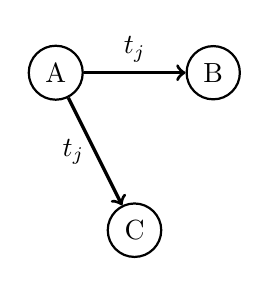
\begin{tikzpicture}
						\begin{scope}[every node/.style={circle,thick,draw}]
							\node (A) at (0,2) {A};
							\node (B) at (2,2) {B};
							\node (C) at (1,0) {C};
						\end{scope}
						
						\begin{scope}[every edge/.style={draw=black,very thick}]
							\path [->] (A) edge node [above] {$t_j$} (B);
							\path [->] (A) edge node [left] {$t_j$} (C);
						\end{scope}
					\end{tikzpicture}
					\caption{Event $(A,\{B,C\},t_j)$}
				\end{subfigure}
				\hfill
				\begin{subfigure}[t]{0.45\linewidth}
					\vskip 0pt
					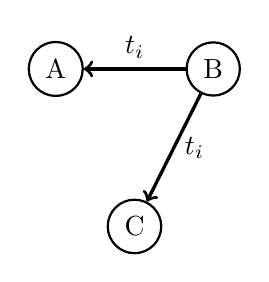
\begin{tikzpicture}
						\begin{scope}[every node/.style={circle,thick,draw}]
							\node (A) at (0,2) {A};
							\node (B) at (2,2) {B};
							\node (C) at (1,0) {C};
						\end{scope}
						
						\begin{scope}[every edge/.style={draw=black,very thick}]
							\path [->] (B) edge node [above] {$t_i$} (A);
							\path [->] (B) edge node [right] {$t_i$} (C);
						\end{scope}
					\end{tikzpicture}
					\caption{Event $(B,\{A,C\},t_i)$}
				\end{subfigure}
				\caption{Illustration of unordered repetition in relational hypereventevent models. Time ordering is $t_j < t_i$.}
				\label{fig:rhem_unordered_repetition}
			\end{mdframed}
		\end{figure}
	
		\item Partial repetition, i.e. the influence of the number of past events $e(h',<t_i)$ on the likelihood of a possible event $e(h,t_i)$, where $h' = (u,v'); \: h = (u,v); \: v \cap v' \neq \emptyset$ $\rightarrow$ is the likelihood of a future event $e(h,t_i)$ associated with the number of past events for which the target sets contain common actors? 
		\begin{align*}
			partial.repetition(e(h,t_i)) = \sum e(h',<t_i); \: h.source = h'.source \land h.targets \cap h'.targets \neq \emptyset
		\end{align*}
		\begin{figure}
			\begin{mdframed}
				\centering
				\begin{subfigure}[t]{0.45\linewidth}
					\vskip 0pt
					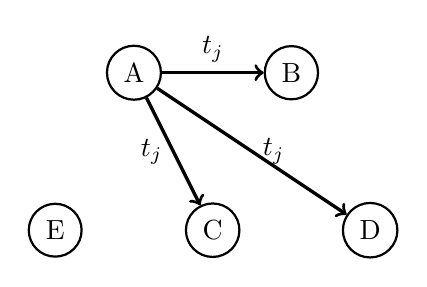
\begin{tikzpicture}
						\begin{scope}[every node/.style={circle,thick,draw}]
							\node (A) at (0,2) {A};
							\node (B) at (2,2) {B};
							\node (C) at (1,0) {C};
							\node (D) at (3,0) {D};
							\node (E) at (-1,0) {E};
						\end{scope}
						
						\begin{scope}[every edge/.style={draw=black,very thick}]
							\path [->] (A) edge node [above] {$t_j$} (B);
							\path [->] (A) edge node [left] {$t_j$} (C);
							\path [->] (A) edge node [right] {$t_j$} (D);
						\end{scope}
					\end{tikzpicture}
					\caption{Event $(A,\{B,C,D\},t_j)$}
				\end{subfigure}
				\hfill
				\begin{subfigure}[t]{0.45\linewidth}
					\vskip 0pt
					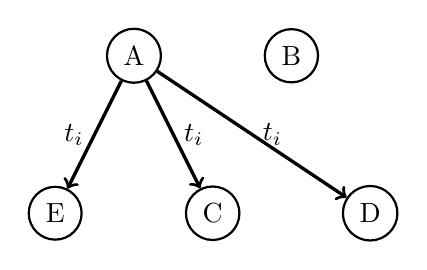
\begin{tikzpicture}
						\begin{scope}[every node/.style={circle,thick,draw}]
							\node (A) at (0,2) {A};
							\node (B) at (2,2) {B};
							\node (C) at (1,0) {C};
							\node (D) at (3,0) {D};
							\node (E) at (-1,0) {E};
						\end{scope}
						
						\begin{scope}[every edge/.style={draw=black,very thick}]
							\path [->] (A) edge node [right] {$t_i$} (C);
							\path [->] (A) edge node [right] {$t_i$} (D);
							\path [->] (A) edge node [left] {$t_i$} (E);
						\end{scope}
					\end{tikzpicture}
					\caption{Event $(A,\{C,D,E\},t_i)$}
				\end{subfigure}
				\caption{Illustration of partial repetition in relational hypereventevent models. Time ordering is $t_j < t_i$.}
				\label{fig:rhem_partial_repetition}
			\end{mdframed}
		\end{figure}
		
		\item Unordered partial repetition, i.e. the influence of past events $e(h',<t_i)$ on the likelihood of a possible event $e(h,t_i)$, where $h' \cap h \neq \emptyset$ $\rightarrow$ is the likelihood of a future event $e(h,t_i)$ associated with the number of past events on hyperedges which contain at least a subset of the same actors, but not necessarily in the same roles?
		\begin{align*}
			unordered.partial.repetition(e(h,t_i)) = \sum e(h',<t_i); \: h \cap h' \neq \emptyset
		\end{align*}
		\begin{figure}
			\begin{mdframed}
				\centering
				\begin{subfigure}[t]{0.45\linewidth}
					\vskip 0pt
					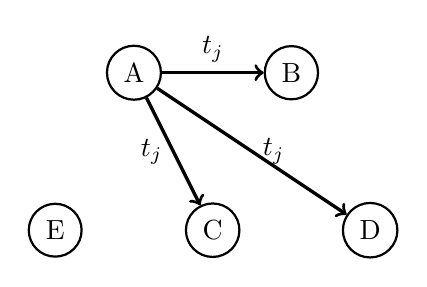
\begin{tikzpicture}
						\begin{scope}[every node/.style={circle,thick,draw}]
							\node (A) at (0,2) {A};
							\node (B) at (2,2) {B};
							\node (C) at (1,0) {C};
							\node (D) at (3,0) {D};
							\node (E) at (-1,0) {E};
						\end{scope}
						
						\begin{scope}[every edge/.style={draw=black,very thick}]
							\path [->] (A) edge node [above] {$t_j$} (B);
							\path [->] (A) edge node [left] {$t_j$} (C);
							\path [->] (A) edge node [right] {$t_j$} (D);
						\end{scope}
					\end{tikzpicture}
					\caption{Event $(A,\{B,C,D\},t_j)$}
				\end{subfigure}
				\hfill
				\begin{subfigure}[t]{0.45\linewidth}
					\vskip 0pt
					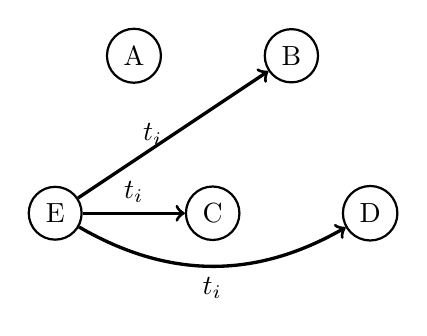
\begin{tikzpicture}
						\begin{scope}[every node/.style={circle,thick,draw}]
							\node (A) at (0,2) {A};
							\node (B) at (2,2) {B};
							\node (C) at (1,0) {C};
							\node (D) at (3,0) {D};
							\node (E) at (-1,0) {E};
						\end{scope}
						
						\begin{scope}[every edge/.style={draw=black,very thick}]
							\path [->] (E) edge node [left] {$t_i$} (B);
							\path [->] (E) edge node [above] {$t_i$} (C);
							\path [->] (E) edge [bend right] node [below] {$t_i$} (D);
						\end{scope}
					\end{tikzpicture}
					\caption{Event $(E,\{B,C,D\},t_i)$}
				\end{subfigure}
				\caption{Illustration of unordered partial repetition in relational hypereventevent models. Time ordering is $t_j < t_i$.}
				\label{fig:rhem_unordered_partial_repetition}
			\end{mdframed}
		\end{figure}
	
		\item Reciprocation, i.e. the influence of past events $e(h',<t_i)$ on the likelihood of a possible event $e(h,t_i)$, where $h' = (u',v'); \: h = (u,v); \: u \subset v' \land v \cap u' \neq \emptyset$ $\rightarrow$ is the likelihood of a future event $e(h,t_i)$ associated with the number of past events where the source of $e$ was part of the target set, and one of the targets of $e$ was the source?
		\begin{align*}
			reciprocation(e(h,t_i)) = \sum e(h',<t_i); \: h.source \subset h'.targets \land h'.source \subset h.targets
		\end{align*}
		\begin{figure}
			\begin{mdframed}
				\centering
				\begin{subfigure}[t]{0.45\linewidth}
					\vskip 0pt
					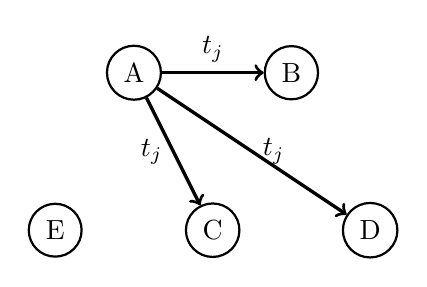
\begin{tikzpicture}
						\begin{scope}[every node/.style={circle,thick,draw}]
							\node (A) at (0,2) {A};
							\node (B) at (2,2) {B};
							\node (C) at (1,0) {C};
							\node (D) at (3,0) {D};
							\node (E) at (-1,0) {E};
						\end{scope}
						
						\begin{scope}[every edge/.style={draw=black,very thick}]
							\path [->] (A) edge node [above] {$t_j$} (B);
							\path [->] (A) edge node [left] {$t_j$} (C);
							\path [->] (A) edge node [right] {$t_j$} (D);
						\end{scope}
					\end{tikzpicture}
					\caption{Event $(A,\{B,C,D\},t_j)$}
				\end{subfigure}
				\hfill
				\begin{subfigure}[t]{0.45\linewidth}
					\vskip 0pt
					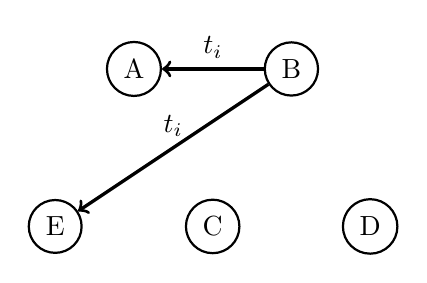
\begin{tikzpicture}
						\begin{scope}[every node/.style={circle,thick,draw}]
							\node (A) at (0,2) {A};
							\node (B) at (2,2) {B};
							\node (C) at (1,0) {C};
							\node (D) at (3,0) {D};
							\node (E) at (-1,0) {E};
						\end{scope}
						
						\begin{scope}[every edge/.style={draw=black,very thick}]
							\path [->] (B) edge node [above] {$t_i$} (A);
							\path [->] (B) edge node [above] {$t_i$} (E);
						\end{scope}
					\end{tikzpicture}
					\caption{Event $(B,\{A,E\},t_i)$}
				\end{subfigure}
				\caption{Illustration of reciprocation in relational hypereventevent models. Time ordering is $t_j < t_i$.}
				\label{fig:rhem_reciprocation}
			\end{mdframed}
		\end{figure}
	
		\item Nominator in-degree, i.e. the influence of past events $e(h',<t_i)$ on the likelihood of a possible event $e(h,t_i)$, where $h' = (u',v'); \: h = (u,v); \: u \subset v' \land v \cap v' = \emptyset$ $\rightarrow$ is the likelihood of a future event $e(h,t_i)$ associated with the number of past events where the source of $e$ was part of the target set, but none of the targets of $e$ was the source?
		\begin{align*}
			&nominator.indegree(e(h,t_i)) = \sum e(h',<t_i);&&\\
			&h.source \subset h'.targets \land h'.source \not\subset h.targets&&
		\end{align*}
		\begin{figure}
			\begin{mdframed}
				\centering
				\begin{subfigure}[t]{0.45\linewidth}
					\vskip 0pt
					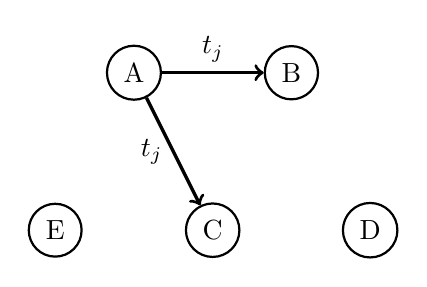
\begin{tikzpicture}
						\begin{scope}[every node/.style={circle,thick,draw}]
							\node (A) at (0,2) {A};
							\node (B) at (2,2) {B};
							\node (C) at (1,0) {C};
							\node (D) at (3,0) {D};
							\node (E) at (-1,0) {E};
						\end{scope}
						
						\begin{scope}[every edge/.style={draw=black,very thick}]
							\path [->] (A) edge node [above] {$t_j$} (B);
							\path [->] (A) edge node [left] {$t_j$} (C);
						\end{scope}
					\end{tikzpicture}
					\caption{Event $(A,\{B,C\},t_j)$}
				\end{subfigure}
				\hfill
				\begin{subfigure}[t]{0.45\linewidth}
					\vskip 0pt
					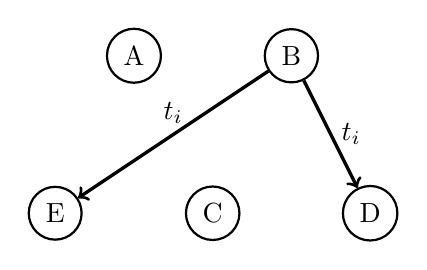
\begin{tikzpicture}
						\begin{scope}[every node/.style={circle,thick,draw}]
							\node (A) at (0,2) {A};
							\node (B) at (2,2) {B};
							\node (C) at (1,0) {C};
							\node (D) at (3,0) {D};
							\node (E) at (-1,0) {E};
						\end{scope}
						
						\begin{scope}[every edge/.style={draw=black,very thick}]
							\path [->] (B) edge node [right] {$t_i$} (D);
							\path [->] (B) edge node [above] {$t_i$} (E);
						\end{scope}
					\end{tikzpicture}
					\caption{Event $(B,\{D,E\},t_i)$}
				\end{subfigure}
				\caption{Illustration of nominator in-degree in relational hypereventevent models. Time ordering is $t_j < t_i$.}
				\label{fig:rhem_nominator_indegree}
			\end{mdframed}
		\end{figure}
	
		\item Nominee out-degree, i.e. the influence of past events $e(h',<t_i)$ on the likelihood of a possible event $e(h,t_i)$, where $h' = (u',v'); \: h = (u,v); \: u' \subset v \land u \not\in v'$ $\rightarrow$ is the likelihood of a future event $e(h,t_i)$ associated with the number of past events where one of the targets of $e$ was the source, but the source of $e$ was none of the targets?
		\begin{align*}
			&nominee.outdegree(e(h,t_i)) = \sum e(h',<t_i);&&\\
			&h'.source \subset h.targets \land h.source \not\subset h'.targets&&
		\end{align*}
		\begin{figure}
			\begin{mdframed}
				\centering
				\begin{subfigure}[t]{0.45\linewidth}
					\vskip 0pt
					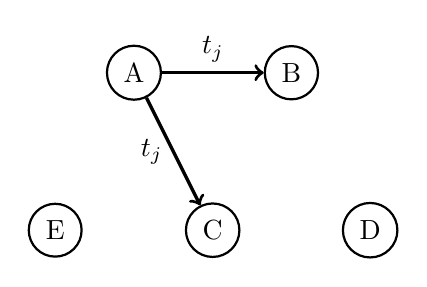
\begin{tikzpicture}
						\begin{scope}[every node/.style={circle,thick,draw}]
							\node (A) at (0,2) {A};
							\node (B) at (2,2) {B};
							\node (C) at (1,0) {C};
							\node (D) at (3,0) {D};
							\node (E) at (-1,0) {E};
						\end{scope}
						
						\begin{scope}[every edge/.style={draw=black,very thick}]
							\path [->] (A) edge node [above] {$t_j$} (B);
							\path [->] (A) edge node [left] {$t_j$} (C);
						\end{scope}
					\end{tikzpicture}
					\caption{Event $(A,\{B,C\},t_j)$}
				\end{subfigure}
				\hfill
				\begin{subfigure}[t]{0.45\linewidth}
					\vskip 0pt
					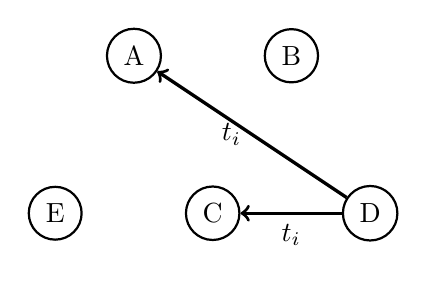
\begin{tikzpicture}
						\begin{scope}[every node/.style={circle,thick,draw}]
							\node (A) at (0,2) {A};
							\node (B) at (2,2) {B};
							\node (C) at (1,0) {C};
							\node (D) at (3,0) {D};
							\node (E) at (-1,0) {E};
						\end{scope}
						
						\begin{scope}[every edge/.style={draw=black,very thick}]
							\path [->] (D) edge node [left] {$t_i$} (A);
							\path [->] (D) edge node [below] {$t_i$} (C);
						\end{scope}
					\end{tikzpicture}
					\caption{Event $(D,\{A,C\},t_i)$}
				\end{subfigure}
				\caption{Illustration of nominee out-degree in relational hypereventevent models. Time ordering is $t_j < t_i$.}
				\label{fig:rhem_nominee_outdegree}
			\end{mdframed}
		\end{figure}
	
		\item Transitive tie, i.e. the influence of past events $e(h',t_j)$ and $e(\text{\emph{\^h}},t_k)$ on the likelihood of a possible event $e(h,t_i)$ ($t_j < t_k < t_i)$, where $h' = (u',v'); \: \text{\emph{\^h}} = (\text{\emph{\^u,\^v}}); \: h = (u,v); \: \text{\emph{\^u}} \subset v' \land v \cap v' \neq \emptyset$ $\rightarrow$ is there a tendency for triadic closure?
		\begin{align*}
			transitive.tie(e(h,t_i)) = \sum_{j \in h.targets} \sum_{a \in \mathcal{A}} \frac{min[d(h.source,\{a\}),d(a,\{j\})]}{\lvert h.targets \rvert}
		\end{align*}
		($\mathcal{A} \setminus \{h.source,j\}$ is the set of all actors $A$ excluding the source actor of $h$ and the iterated actor $j \in h.targets$, and $d(x,y)$ is the accumulated volume of interactions from $x$ to $y$ by the time $t_i$)
		\begin{figure}
			\begin{mdframed}
				\centering
				\begin{subfigure}[t]{0.3\linewidth}
					\vskip 0pt
					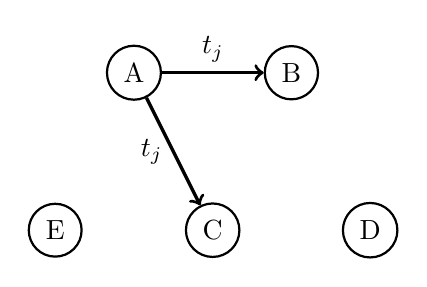
\begin{tikzpicture}
						\begin{scope}[every node/.style={circle,thick,draw}]
							\node (A) at (0,2) {A};
							\node (B) at (2,2) {B};
							\node (C) at (1,0) {C};
							\node (D) at (3,0) {D};
							\node (E) at (-1,0) {E};
						\end{scope}
						
						\begin{scope}[every edge/.style={draw=black,very thick}]
							\path [->] (A) edge node [above] {$t_j$} (B);
							\path [->] (A) edge node [left] {$t_j$} (C);
						\end{scope}
					\end{tikzpicture}
					\caption{Event $(A,\{B,C\},t_j)$}
				\end{subfigure}
				\hfill
				\begin{subfigure}[t]{0.3\linewidth}
					\vskip 0pt
					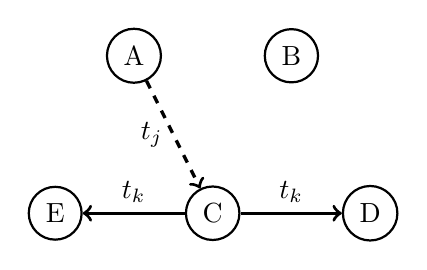
\begin{tikzpicture}
						\begin{scope}[every node/.style={circle,thick,draw}]
							\node (A) at (0,2) {A};
							\node (B) at (2,2) {B};
							\node (C) at (1,0) {C};
							\node (D) at (3,0) {D};
							\node (E) at (-1,0) {E};
						\end{scope}
						
						\begin{scope}[every edge/.style={draw=black,very thick}]
							\path [->] (A) edge [dashed] node [left] {$t_j$} (C);
							\path [->] (C) edge node [above] {$t_k$} (D);
							\path [->] (C) edge node [above] {$t_k$} (E);
						\end{scope}
					\end{tikzpicture}
					\caption{Event $(C,\{D,E\},t_i)$}
				\end{subfigure}
				\hfill
				\begin{subfigure}[t]{0.3\linewidth}
					\vskip 0pt
					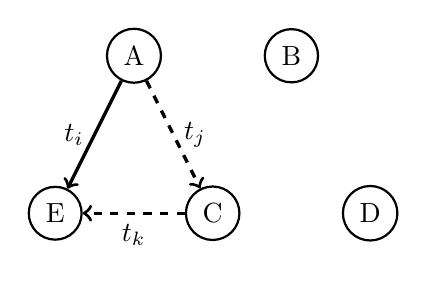
\begin{tikzpicture}
						\begin{scope}[every node/.style={circle,thick,draw}]
							\node (A) at (0,2) {A};
							\node (B) at (2,2) {B};
							\node (C) at (1,0) {C};
							\node (D) at (3,0) {D};
							\node (E) at (-1,0) {E};
						\end{scope}
						
						\begin{scope}[every edge/.style={draw=black,very thick}]
							\path [->] (A) edge [dashed] node [right] {$t_j$} (C);
							\path [->] (C) edge [dashed] node [below] {$t_k$} (E);
							\path [->] (A) edge node [left] {$t_i$} (E);
							%\path [->] (B) edge node [above] {$t_i$} (E);
						\end{scope}
					\end{tikzpicture}
					\caption{Event $(A,\{E\},t_i)$}
				\end{subfigure}
				\caption{Illustration of transitive tie in relational hypereventevent models. Time ordering is $t_j < t_k < t_i$. Dashed lines represent previous edges relevant to the closure.}
				\label{fig:rhem_transitive_tie}
			\end{mdframed}
		\end{figure}
	
		\item Cyclical tie, i.e. the influence of past events $e(h',t_j)$ and $e(\text{\emph{\^h}},t_k)$ on the likelihood of a possible event $e(h,t_i)$ ($t_j < t_k < t_i)$, where $h' = (u',v'); \: \text{\emph{\^h}} = (\text{\emph{\^u,\^v}}); \: h = (u,v); \: \text{\emph{\^u}} \subset v' \land u' \subset v$ $\rightarrow$ is there a tendency for cyclic closure?
		\begin{align*}
			cyclical.tie(e(h,t_i)) = \sum_{j \in h.targets} \sum_{a \in \mathcal{A}} \frac{min[d(a,\{h.source\}),d(j,\{a\})]}{\lvert h.targets \rvert}
		\end{align*}
		\begin{figure}
			\begin{mdframed}
				\centering
				\begin{subfigure}[t]{0.3\linewidth}
					\vskip 0pt
					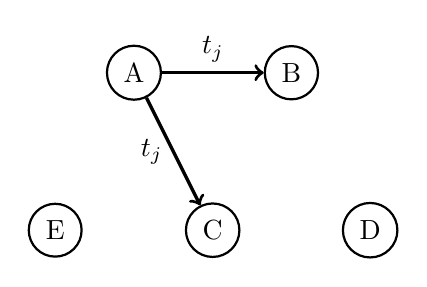
\begin{tikzpicture}
						\begin{scope}[every node/.style={circle,thick,draw}]
							\node (A) at (0,2) {A};
							\node (B) at (2,2) {B};
							\node (C) at (1,0) {C};
							\node (D) at (3,0) {D};
							\node (E) at (-1,0) {E};
						\end{scope}
						
						\begin{scope}[every edge/.style={draw=black,very thick}]
							\path [->] (A) edge node [above] {$t_j$} (B);
							\path [->] (A) edge node [left] {$t_j$} (C);
						\end{scope}
					\end{tikzpicture}
					\caption{Event $(A,\{B,C\},t_j)$}
				\end{subfigure}
				\hfill
				\begin{subfigure}[t]{0.3\linewidth}
					\vskip 0pt
					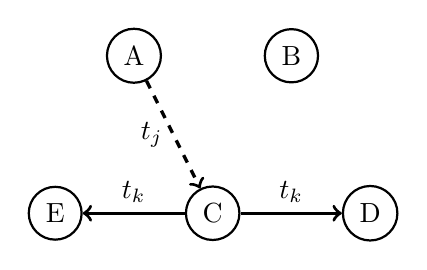
\begin{tikzpicture}
						\begin{scope}[every node/.style={circle,thick,draw}]
							\node (A) at (0,2) {A};
							\node (B) at (2,2) {B};
							\node (C) at (1,0) {C};
							\node (D) at (3,0) {D};
							\node (E) at (-1,0) {E};
						\end{scope}
						
						\begin{scope}[every edge/.style={draw=black,very thick}]
							\path [->] (A) edge [dashed] node [left] {$t_j$} (C);
							\path [->] (C) edge node [above] {$t_k$} (D);
							\path [->] (C) edge node [above] {$t_k$} (E);
						\end{scope}
					\end{tikzpicture}
					\caption{Event $(C,\{D,E\},t_i)$}
				\end{subfigure}
				\hfill
				\begin{subfigure}[t]{0.3\linewidth}
					\vskip 0pt
					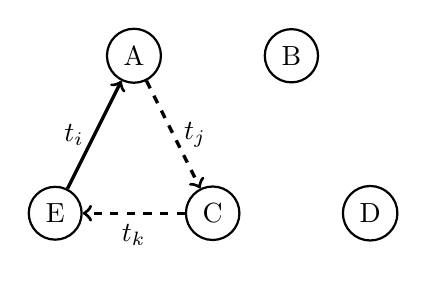
\begin{tikzpicture}
						\begin{scope}[every node/.style={circle,thick,draw}]
							\node (A) at (0,2) {A};
							\node (B) at (2,2) {B};
							\node (C) at (1,0) {C};
							\node (D) at (3,0) {D};
							\node (E) at (-1,0) {E};
						\end{scope}
						
						\begin{scope}[every edge/.style={draw=black,very thick}]
							\path [->] (A) edge [dashed] node [right] {$t_j$} (C);
							\path [->] (C) edge [dashed] node [below] {$t_k$} (E);
							\path [->] (E) edge node [left] {$t_i$} (A);
							%\path [->] (B) edge node [above] {$t_i$} (E);
						\end{scope}
					\end{tikzpicture}
					\caption{Event $(E,\{A\},t_i)$}
				\end{subfigure}
				\caption{Illustration of cyclical tie in relational hypereventevent models. Time ordering is $t_j < t_k < t_i$. Dashed lines represent previous edges relevant to the closure.}
				\label{fig:rhem_cyclical_tie}
				\end{mdframed}
			\end{figure}
		
			\item Shared source, i.e. the influence of past events $e(h',t_j)$ and $e(\text{\emph{\^h}},t_k)$ on the likelihood of a possible event $e(h,t_i)$ ($t_j < t_k < t_i)$, where $h' = (u',v'); \: \text{\emph{\^h}} = (\text{\emph{\^u,\^v}}); \: h = (u,v); \: u' = \text{\emph{\^u}} \land u \subset v' \land v \cap \text{\emph{\^v}} \neq \emptyset$ $\rightarrow$ are actors who were targets of the same source in previous events more likely to interact?
			\begin{align*}
				shared.source(e(h,t_i)) = \sum_{j \in h.targets} \sum_{a \in \mathcal{A}} \frac{min[d(a,\{h.source\}),d(a,\{j\})]}{\lvert h.targets \rvert}
			\end{align*}
			\begin{figure}
				\begin{mdframed}
					\centering
					\begin{subfigure}[t]{0.3\linewidth}
						\vskip 0pt
						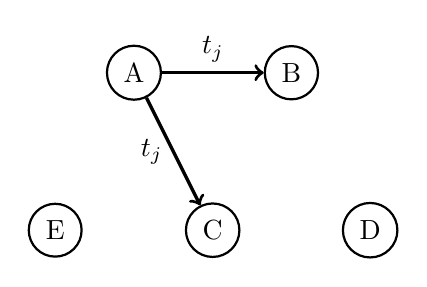
\begin{tikzpicture}
							\begin{scope}[every node/.style={circle,thick,draw}]
								\node (A) at (0,2) {A};
								\node (B) at (2,2) {B};
								\node (C) at (1,0) {C};
								\node (D) at (3,0) {D};
								\node (E) at (-1,0) {E};
							\end{scope}
							
							\begin{scope}[every edge/.style={draw=black,very thick}]
								\path [->] (A) edge node [above] {$t_j$} (B);
								\path [->] (A) edge node [left] {$t_j$} (C);
							\end{scope}
						\end{tikzpicture}
						\caption{Event $(A,\{B,C\},t_j)$}
					\end{subfigure}
					\hfill
					\begin{subfigure}[t]{0.3\linewidth}
						\vskip 0pt
						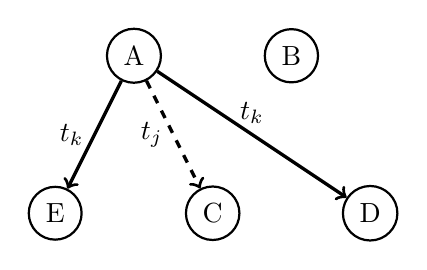
\begin{tikzpicture}
							\begin{scope}[every node/.style={circle,thick,draw}]
								\node (A) at (0,2) {A};
								\node (B) at (2,2) {B};
								\node (C) at (1,0) {C};
								\node (D) at (3,0) {D};
								\node (E) at (-1,0) {E};
							\end{scope}
							
							\begin{scope}[every edge/.style={draw=black,very thick}]
								\path [->] (A) edge [dashed] node [left] {$t_j$} (C);
								\path [->] (A) edge node [above] {$t_k$} (D);
								\path [->] (A) edge node [left] {$t_k$} (E);
							\end{scope}
						\end{tikzpicture}
						\caption{Event $(A,\{D,E\},t_i)$}
					\end{subfigure}
					\hfill
					\begin{subfigure}[t]{0.3\linewidth}
						\vskip 0pt
						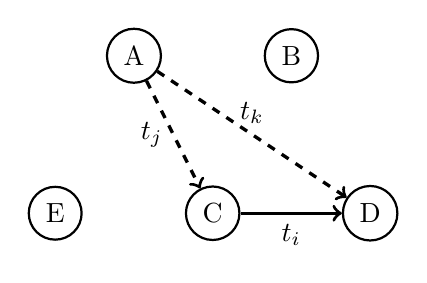
\begin{tikzpicture}
							\begin{scope}[every node/.style={circle,thick,draw}]
								\node (A) at (0,2) {A};
								\node (B) at (2,2) {B};
								\node (C) at (1,0) {C};
								\node (D) at (3,0) {D};
								\node (E) at (-1,0) {E};
							\end{scope}
							
							\begin{scope}[every edge/.style={draw=black,very thick}]
								\path [->] (A) edge [dashed] node [left] {$t_j$} (C);
								\path [->] (A) edge [dashed] node [above] {$t_k$} (D);
								\path [->] (C) edge node [below] {$t_i$} (D);
								%\path [->] (B) edge node [above] {$t_i$} (E);
							\end{scope}
						\end{tikzpicture}
						\caption{Event $(C,\{D\},t_i)$}
					\end{subfigure}
					\caption{Illustration of shared source in relational hypereventevent models. Time ordering is $t_j < t_k < t_i$. Dashed lines represent previous edges relevant to the closure.}
					\label{fig:rhem_shared_source}
				\end{mdframed}
		\end{figure}
	
		\item Shared target, i.e. the influence of past events $e(h',t_j)$ and $e(\text{\emph{\^h}},t_k)$ on the likelihood of a possible event $e(h,t_i)$ ($t_j < t_k < t_i)$, where $h' = (u',v'); \: \text{\emph{\^h}} = (\text{\emph{\^u,\^v}}); \: h = (u,v); \: v' \cap \text{\emph{\^v}} \neq \emptyset \land u = u' \land \text{\emph{\^u}} \subset v$ $\rightarrow$ are actors who targeted the same actors in previous events more likely to interact?
		\begin{align*}
			shared.target(e(h,t_i)) = \sum_{j \in h.targets} \sum_{a \in \mathcal{A}} \frac{min[d(h.source,\{a\}),d(j,\{a\})]}{\lvert h.targets \rvert}
		\end{align*}
		\begin{figure}
			\begin{mdframed}
				\centering
				\begin{subfigure}[t]{0.3\linewidth}
					\vskip 0pt
					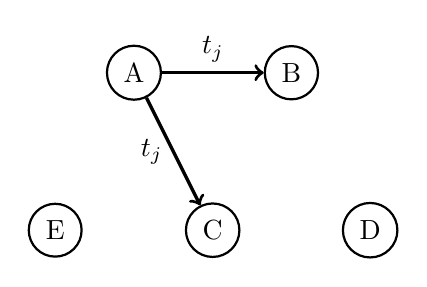
\begin{tikzpicture}
						\begin{scope}[every node/.style={circle,thick,draw}]
							\node (A) at (0,2) {A};
							\node (B) at (2,2) {B};
							\node (C) at (1,0) {C};
							\node (D) at (3,0) {D};
							\node (E) at (-1,0) {E};
						\end{scope}
						
						\begin{scope}[every edge/.style={draw=black,very thick}]
							\path [->] (A) edge node [above] {$t_j$} (B);
							\path [->] (A) edge node [left] {$t_j$} (C);
						\end{scope}
					\end{tikzpicture}
					\caption{Event $(A,\{B,C\},t_j)$}
				\end{subfigure}
				\hfill
				\begin{subfigure}[t]{0.3\linewidth}
					\vskip 0pt
					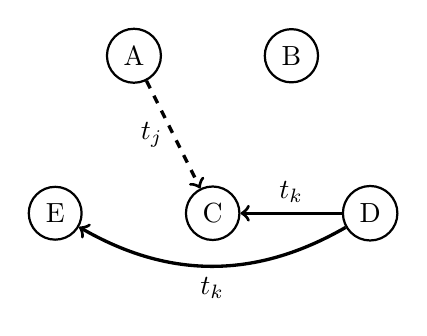
\begin{tikzpicture}
						\begin{scope}[every node/.style={circle,thick,draw}]
							\node (A) at (0,2) {A};
							\node (B) at (2,2) {B};
							\node (C) at (1,0) {C};
							\node (D) at (3,0) {D};
							\node (E) at (-1,0) {E};
						\end{scope}
						
						\begin{scope}[every edge/.style={draw=black,very thick}]
							\path [->] (A) edge [dashed] node [left] {$t_j$} (C);
							\path [->] (D) edge node [above] {$t_k$} (C);
							\path [->] (D) edge [bend left] node [below] {$t_k$} (E);
						\end{scope}
					\end{tikzpicture}
					\caption{Event $(D,\{C,E\},t_i)$}
				\end{subfigure}
				\hfill
				\begin{subfigure}[t]{0.3\linewidth}
					\vskip 0pt
					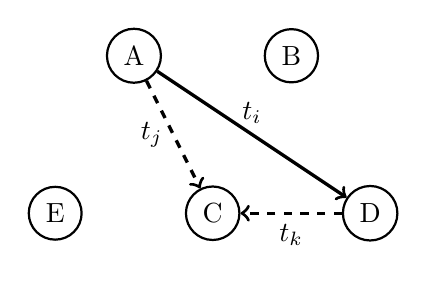
\begin{tikzpicture}
						\begin{scope}[every node/.style={circle,thick,draw}]
							\node (A) at (0,2) {A};
							\node (B) at (2,2) {B};
							\node (C) at (1,0) {C};
							\node (D) at (3,0) {D};
							\node (E) at (-1,0) {E};
						\end{scope}
						
						\begin{scope}[every edge/.style={draw=black,very thick}]
							\path [->] (A) edge [dashed] node [left] {$t_j$} (C);
							\path [->] (D) edge [dashed] node [below] {$t_k$} (C);
							\path [->] (A) edge node [above] {$t_i$} (D);
							%\path [->] (B) edge node [above] {$t_i$} (E);
						\end{scope}
					\end{tikzpicture}
					\caption{Event $(A,\{D\},t_i)$}
				\end{subfigure}
				\caption{Illustration of shared target in relational hypereventevent models. Time ordering is $t_j < t_k < t_i$. Dashed lines represent previous edges relevant to the closure.}
				\label{fig:rhem_shared_target}
			\end{mdframed}
		\end{figure}
	
	\end{itemize}
	\item Effects depending on actor attributes:
	\begin{itemize}
		\item Nominator age
		\item Nominees average age
		\item Nominator-nominees age difference
		\item Nominees age difference
		\item Nominator sex
		\item Nominees average sex
		\item Nominator-nominees sex difference
		\item Nominees sex difference
		\item Other covariates specific to the individual datasets, which are listed in section \ref{ch:previous_work_data}. In general, there are four statistics for each covariate: the value of the nominator, the average value of the nominees, the difference in value between nominator and nominees, and the difference in value between nominees.
	\end{itemize}
\end{itemize}

\noindent These statistics were likewise calculated using the \emph{eventnet} software \cite{eventnet_rem,eventnet_rhem}. Using the \emph{R} package \emph{survival} \cite{survival-package}, a Cox proportional hazards model was fitted on the result tables in order to estimate the model parameters $\theta$, and therefore draw conclusions regarding significance and effect of the individual statistics. Results are presented and discussed in chapter \ref{ch:results_discussion}.

